\chapter{SatNOGS: Глобальная сеть наземных спутниковых станций с открытым исходным кодом}

SatNOGS представляет собой комплексную платформу \cite{satnogs_general_docs},
обеспечивающую функционирование открытой сети наземных станций для мониторинга
спутников. Основной целью проекта является разработка полного стека открытых
технологий, основанных на открытых стандартах, и создание полноценной наземной
станции в качестве демонстрации возможностей данного стека.

Система SatNOGS способна принимать сигналы со спутников, находящихся на низкой
околоземной орбите (LEO), в диапазонах UHF и VHF. Она позволяет извлекать
сигналы состояния и телеметрии, данные с научных и исследовательских спутников
(например, результаты магнитосферных экспериментов), метеорологические данные и
другую информацию.

Проект SatNOGS включает в себя несколько ключевых компонентов: веб-приложение
для планирования наблюдений, базу данных для хранения информации о спутниках,
клиентское программное обеспечение для работы на наземных станциях и аппаратное
обеспечение с открытым исходным кодом. Все это создает модульную архитектуру,
позволяющую легко интегрировать новые функции и расширять функциональность
системы.

SatNOGS активно развивает сообщество пользователей и разработчиков, предлагая
доступ к документации и инструментам для создания собственных наземных станций.
Это создает возможности для участия в глобальной сети наблюдений за спутниками
и обмена данными между участниками проекта.

\section{Компоненты SatNOGS}

SatNOGS включает в себя несколько ключевых компонентов, каждый из которых
играет важную роль в функционировании платформы, см. рисунок
\ref{fig:satnogs_data_flow}.
Ниже представлена таблица, описывающая основные элементы системы:

\begin{table}[h]
	\centering
	\begin{tabular}{|l|p{10cm}|}
		\hline \textbf{Компонент} & \textbf{Описание}
		\\ \hline SatNOGS Network          & Веб-приложение, предназначенное для
		планирования наблюдений по сети наземных станций. Оно способствует
		координации наблюдений за спутниковыми сигналами и планированию таких
		наблюдений среди наземных станций, подключенных к сети.                                 \\ \hline База
		данных SatNOGS            & Ресурс, позволяющий пользователям предоставлять
		информацию о передатчиках активных спутников. Данные доступны через API или
		веб-интерфейс.
		\\ \hline Клиент SatNOGS           & Программное обеспечение, работающее на
		наземных станциях (обычно на встраиваемых системах). Оно получает
		регулярные задания на наблюдение из сети, принимает спутниковые передачи и
		отправляет их обратно в веб-приложение Network.                                         \\ \hline Наземная станция
		SatNOGS                   & Аппаратное обеспечение наземной станции с открытым исходным
		кодом, включающее ротаторы, антенны и электронику, подключенные к клиенту.
		\\ \hline SatNOGS Dashboard        & Веб-интерфейс для визуализации и
		анализа данных телеметрии, полученных от спутников. Он предоставляет
		пользователям возможность отслеживать состояние спутников и их сигналы в
		реальном времени.                                                                       \\ \hline
	\end{tabular}
	\caption{Основные компоненты системы SatNOGS}
	\label{tab:satnogs_components}
\end{table}

Система SatNOGS активно развивает сообщество пользователей и разработчиков,
предлагая доступ к документации и инструментам для создания собственных
наземных станций. Это создает возможности для участия в глобальной сети
наблюдений за спутниками и обмена данными между участниками проекта.

\begin{figure}[htbp]
	\centering
	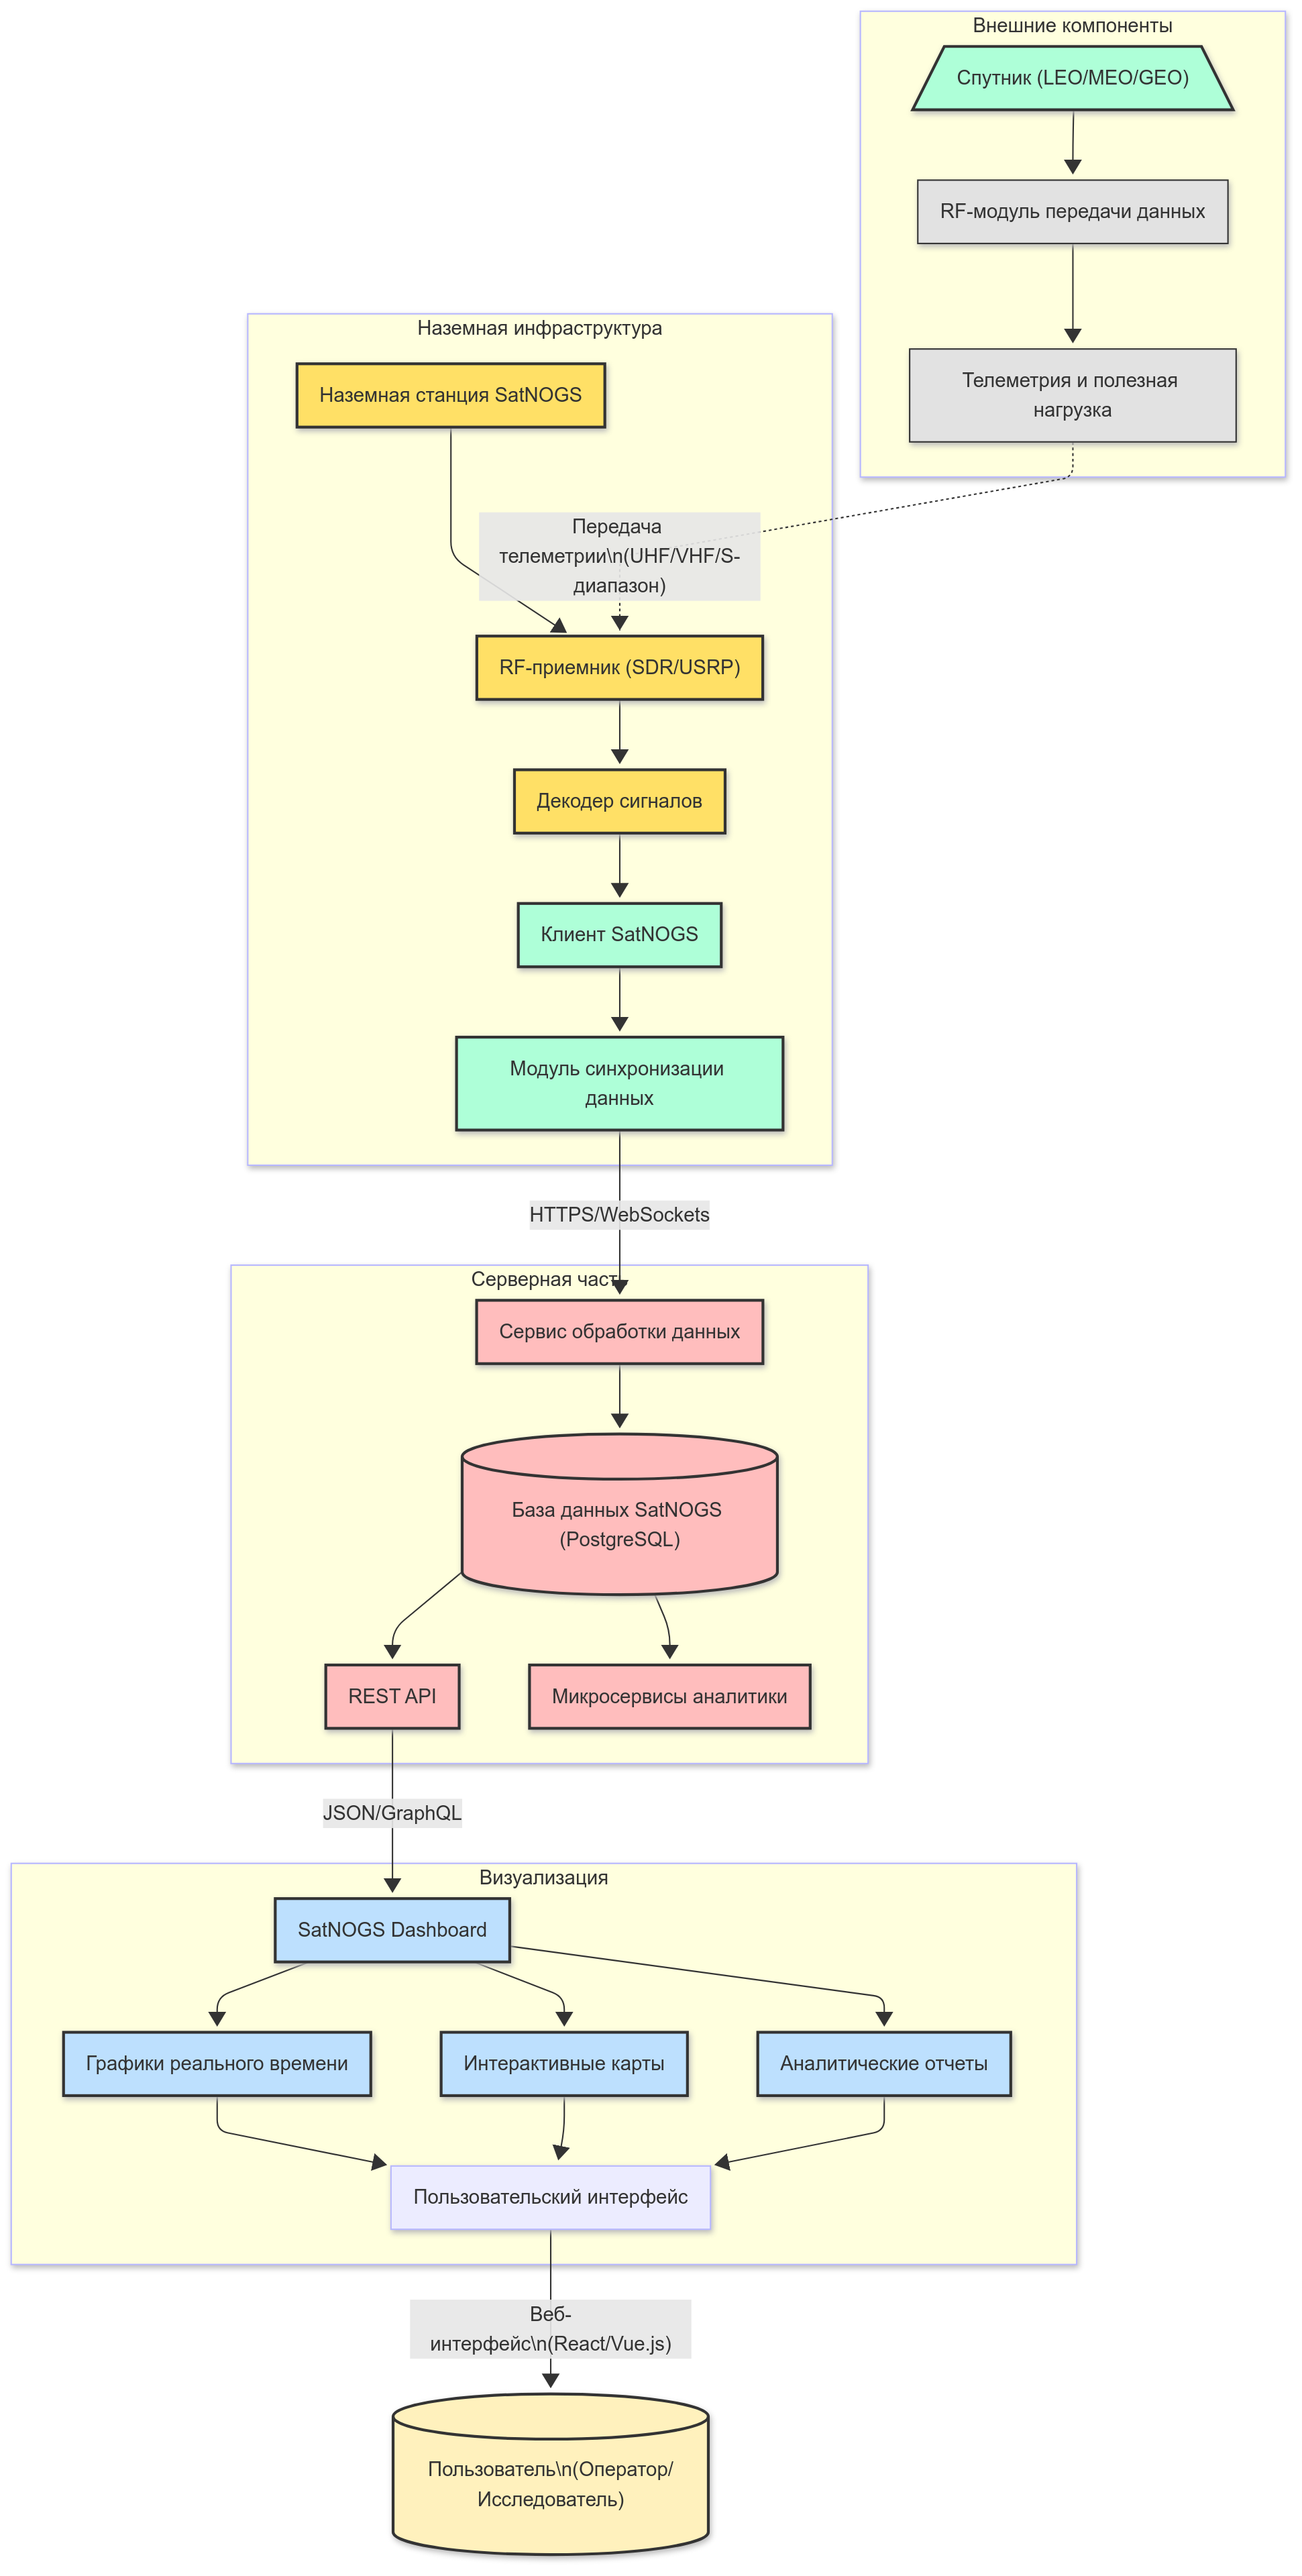
\includegraphics[width=0.7\textwidth]{satnogs_data_flow}
	\caption{Поток данных SatNOGS в Dashboard endpoint}
	\label{fig:satnogs_data_flow}
\end{figure}

\section{SatNOGS Dashboard}

\begin{figure}[htbp]
	\centering
	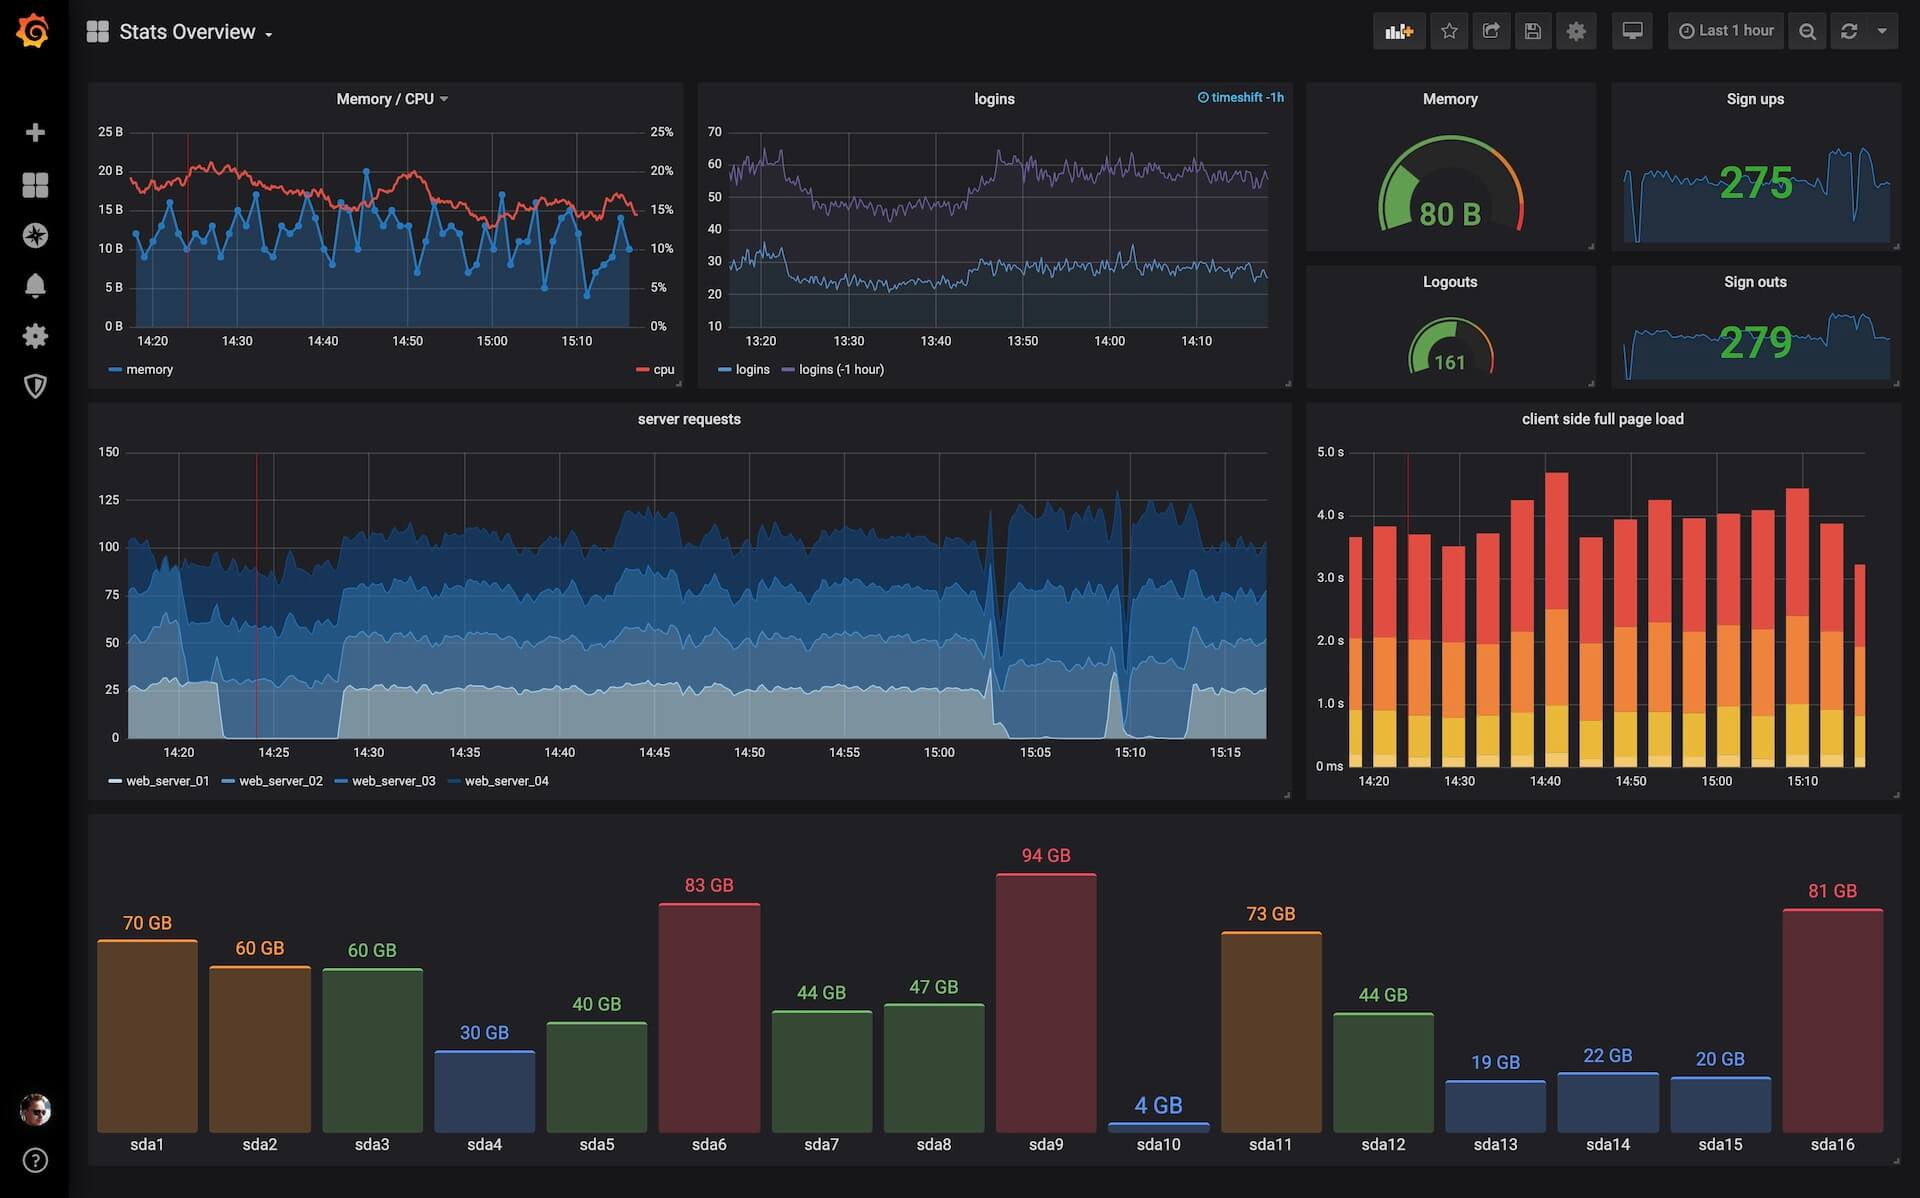
\includegraphics[width=1.0\textwidth]{grafana_example}
	\caption{Пример страницы с данными в Grafana Enterprise}
	\label{fig:grafana_example}
\end{figure}

SatNOGS Dashboard представляет собой ключевой компонент в нашей
исследовательской работе, выступая в качестве основного источника данных для
обучения моделей. После детального анализа архитектуры системы было определено
оптимальное место для извлечения данных. Dashboard Grafana в рамках экосистемы
SatNOGS предоставляет уже предобработанные данные, прошедшие фильтрацию и
дедупликацию посредством построения временных рядов. Несмотря на то, что
система содержит информацию только о приблизительно 120 спутниках, этот объем
является достаточным для анализа критических метрик и позволяет существенно
сократить затраты времени и вычислительных ресурсов на обучение, при этом
обеспечивая независимость от инфраструктуры SatNOGS.

Grafana — это мощная платформа для визуализации и анализа данных, которая
позволяет создавать интерактивные дашборды на основе различных источников
данных \cite{grafana_docs}. Пример такого дашборда можно увидеть на рисунке
\ref{fig:grafana_example}.
Grafana широко используется для мониторинга систем и приложений, предоставляя
пользователям возможность отслеживать ключевые метрики в реальном времени.

В контексте SatNOGS Dashboard, Grafana работает с базой данных
\textbf{InfluxDB} \cite{influxdb_docs}, которая предназначена для хранения
временных рядов данных, таких как телеметрия спутников. Данные поступают от
наземных станций, обрабатываются клиентом SatNOGS и сохраняются в InfluxDB.
Затем Grafana использует API для доступа к этим данным и их визуализации на
дашбордах.

Однако стоит отметить, что доступ к API Grafana Dashboard SatNOGS был закрыт,
что ограничивает возможности пользователей в получении данных напрямую. Более
того, Grafana не предоставляет свои услуги пользователям из России и Беларуси в
связи с санциями \cite{grafana_community_post}, что создает дополнительные
сложности для разработчиков и исследователей из этих стран. Это делает Grafana
ненадежной платформой для работы в нашем регионе.

В ответ на эти ограничения нами разрабатывается специализированный парсер для
обхода существующих барьеров и получения необходимых данных. Данный инструмент
будет подробно рассмотрен в последующих разделах работы, поскольку он является
ключевым компонентом для интеграции данных из SatNOGS Dashboard в нашу систему
анализа и визуализации.

Таким образом, несмотря на значительный потенциал Grafana как инструмента
визуализации, текущие ограничения доступа существенно снижают её практическую
ценность для пользователей из определённых регионов, что обуславливает
необходимость разработки альтернативных методов работы с данными.
Схему работы SatNOGS Dashboard можно наблюдать на рисунке
\ref{fig:grafana_infra}.

\begin{figure}[htbp]
	\centering
	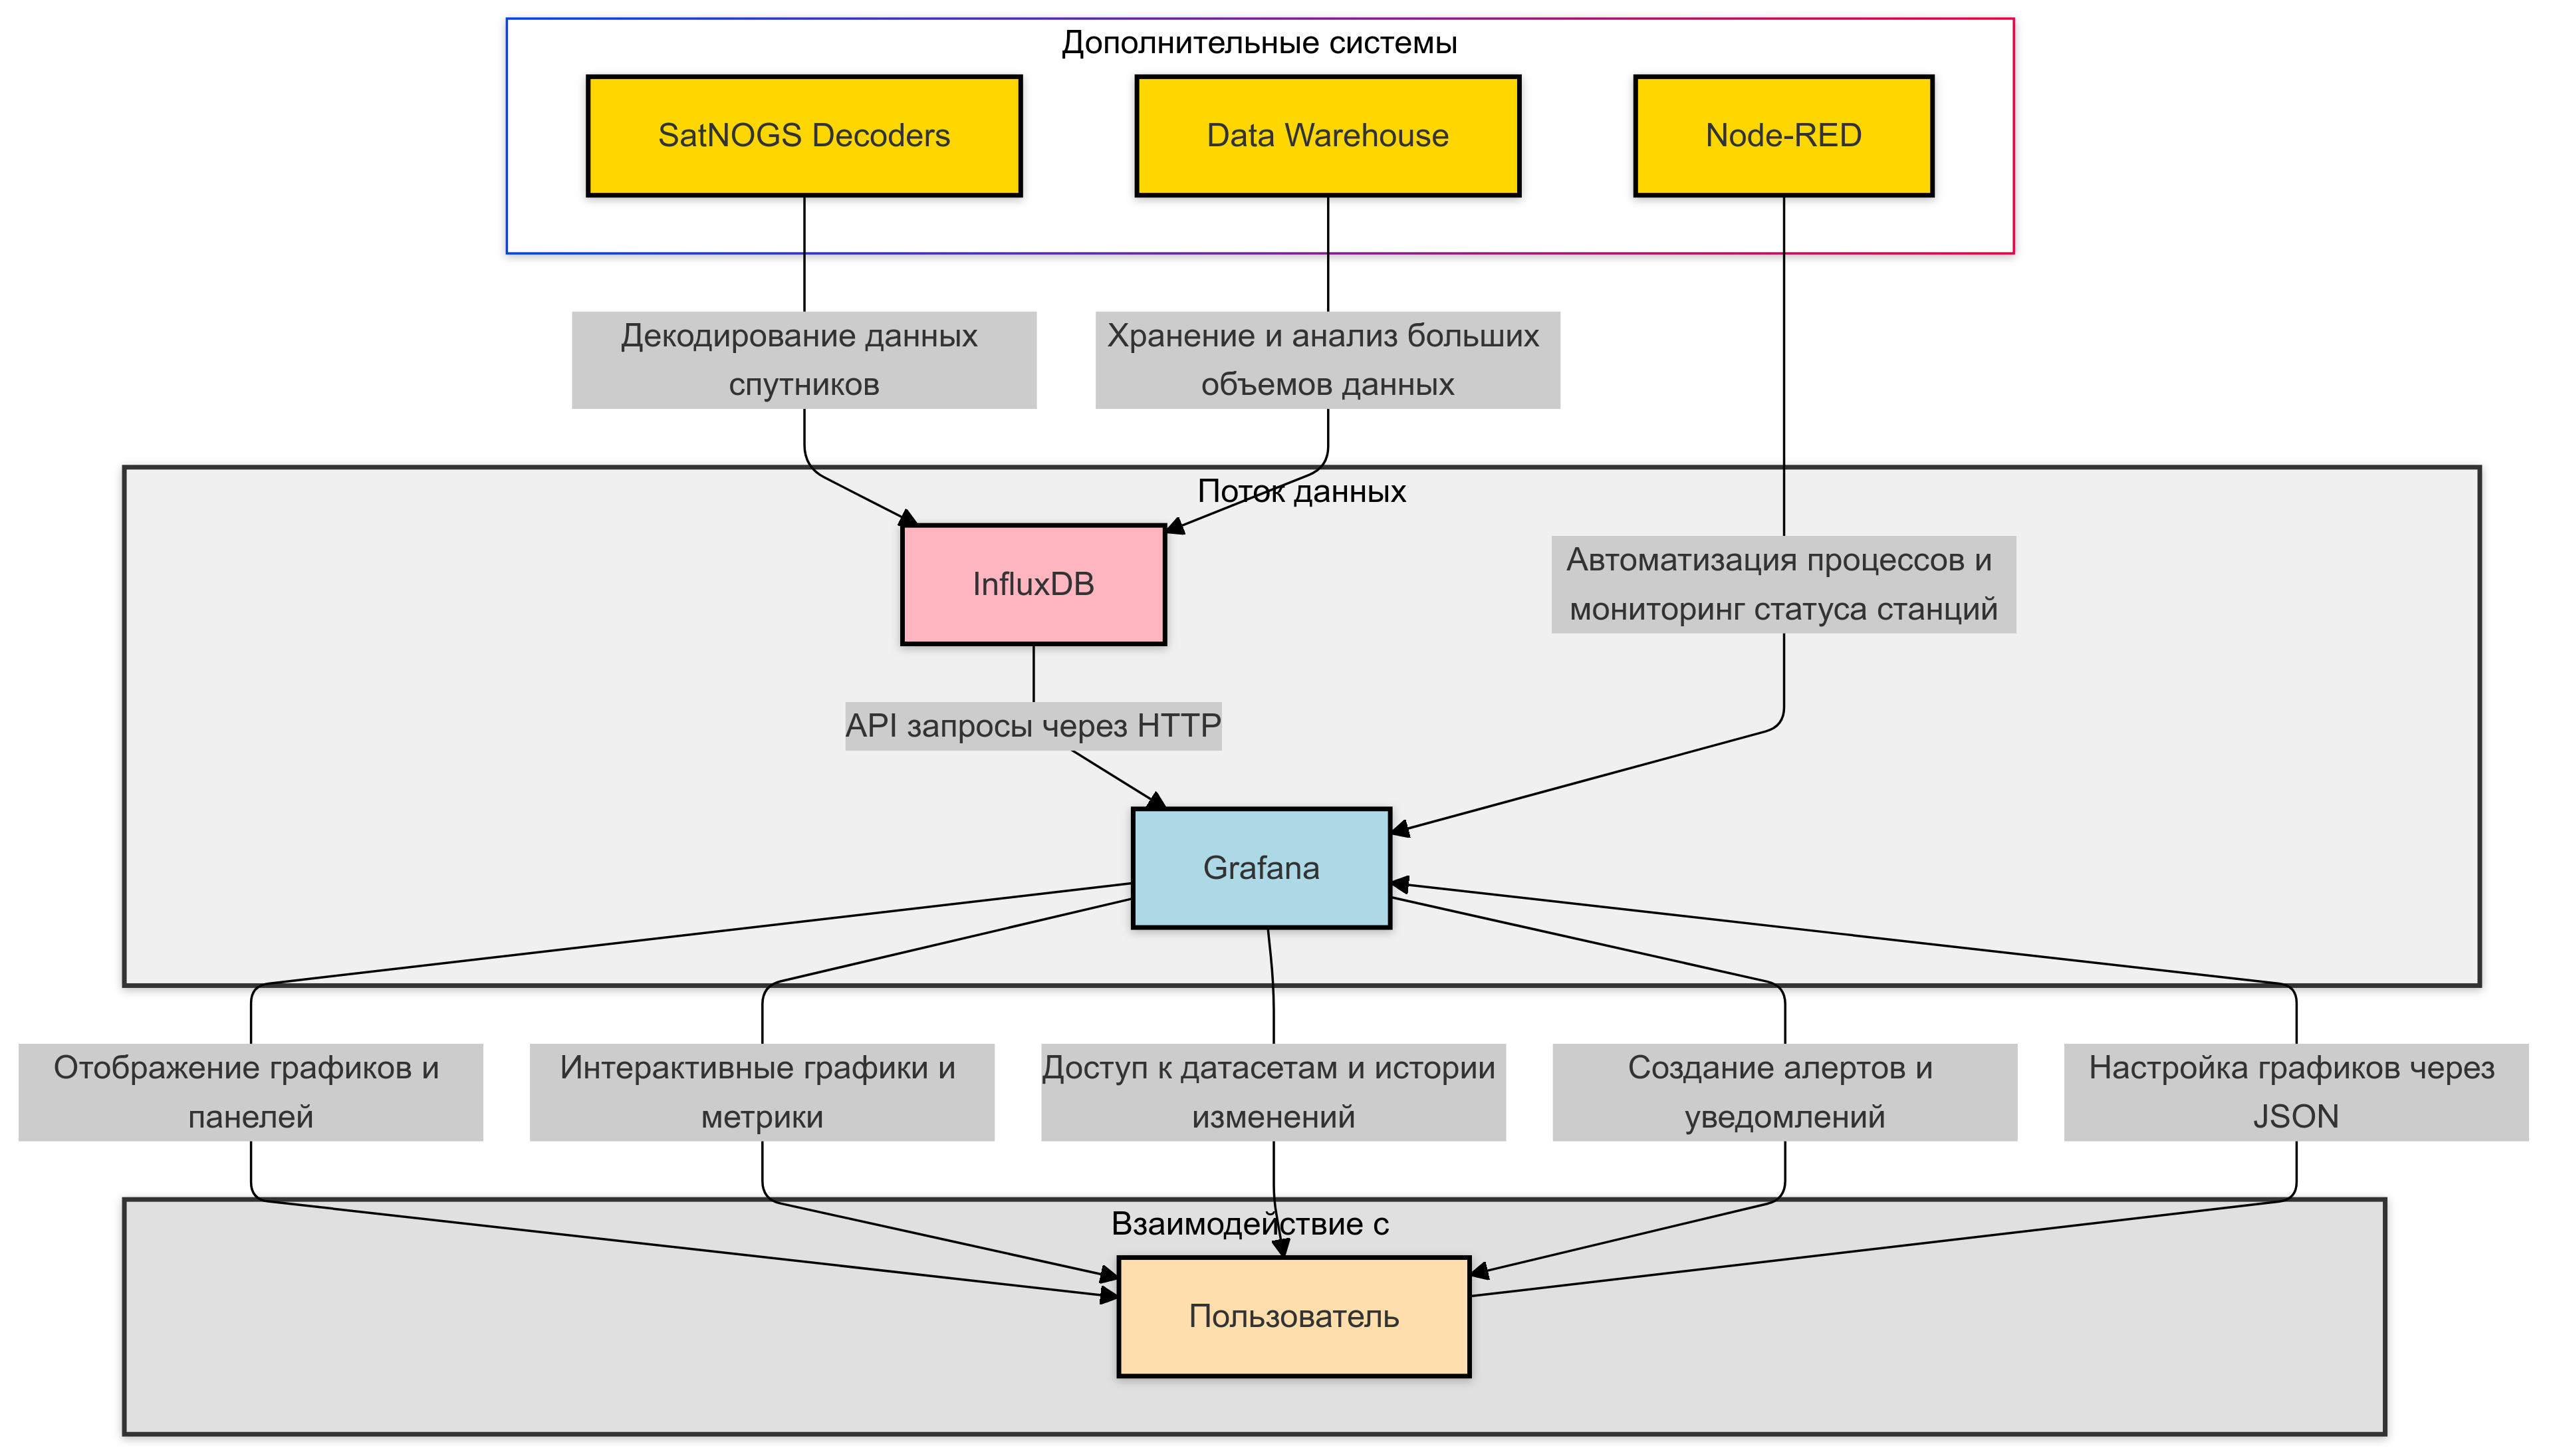
\includegraphics[width=1.0\textwidth]{grafana_infra}
	\caption{Подробное устройство SatNOGS Dashboard}
	\label{fig:grafana_infra}
\end{figure}

\subsection{Устройство frontend SatNOGS Dashboard}
\begin{figure}[htbp]
	\centering
	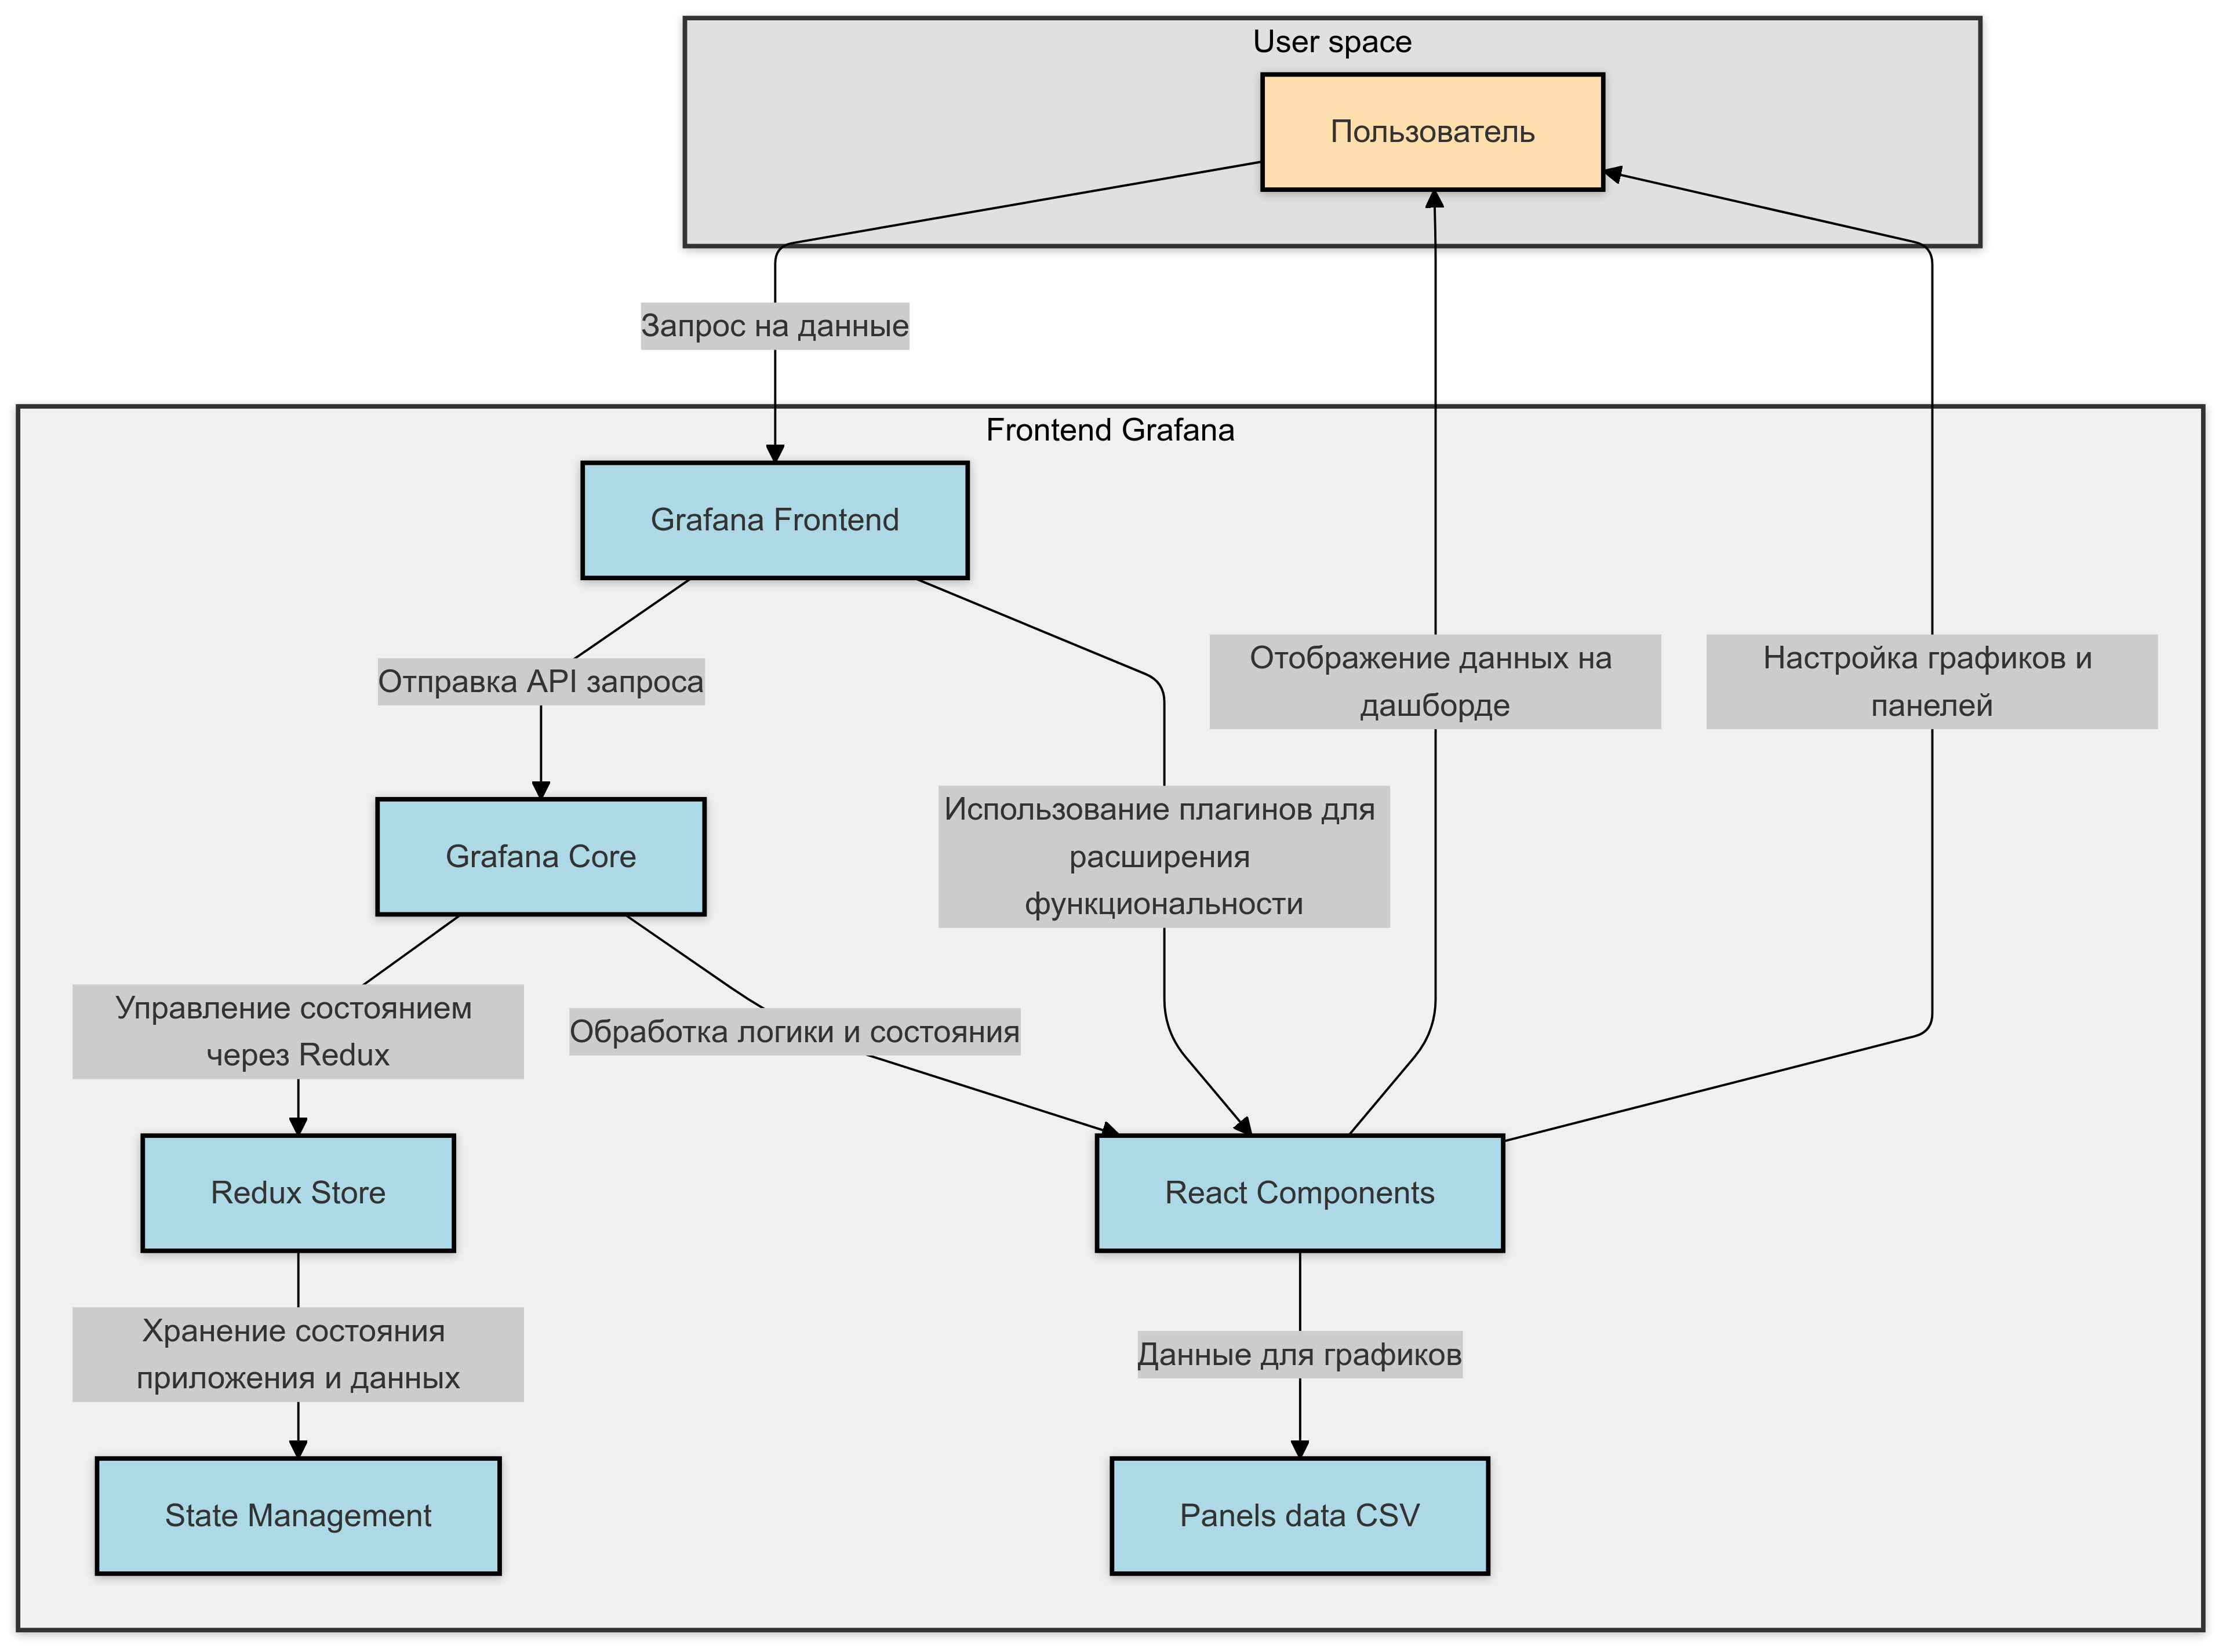
\includegraphics[width=1.0\textwidth]{grafana_frontend_structure}
	\caption{Построение frontend части grafana \cite{react_managing_state}}
	\label{fig:grafana_frontend_structure}
\end{figure}

Разберем схему архитектуры фронтенд-части системы
\ref{fig:grafana_frontend_structure}
Grafana.
Данная схема иллюстрирует взаимодействие компонентов пользовательского
интерфейса Grafana и потоки данных между ними.

Архитектура построена по многоуровневому принципу, где пользовательское
пространство (User space) взаимодействует с фронтенд-частью Grafana через
запросы на получение данных. Фронтенд Grafana состоит из нескольких ключевых
компонентов: Grafana Frontend, Grafana Core, Redux Store, State Management,
React Components и Panels data CSV.

Процесс работы системы начинается с запроса пользователя на получение данных,
который обрабатывается компонентом Grafana Frontend. Этот компонент отправляет
API-запросы к Grafana Core, который выполняет обработку логики и состояния.
Grafana Core взаимодействует с Redux Store для управления состоянием приложения
через механизм Redux. State Management отвечает за хранение состояния
приложения и данных.

React Components играют центральную роль в системе, обеспечивая отображение
данных на дашборде, настройку графиков и панелей, а также расширение
функциональности через плагины. Компонент Panels data CSV отвечает за
подготовку данных для графиков.

Для эффективного парсинга данной системы следует сосредоточиться на компоненте
Panels data CSV, который содержит структурированные данные для визуализации, а
также на API-запросах между Grafana Frontend и Grafana Core. Стратегия парсинга
должна учитывать, что данные проходят через несколько уровней обработки,
включая React Components, и хранятся в Redux Store. Понимание этой архитектуры
позволяет определить оптимальные точки извлечения данных и методы обхода
возможных ограничений доступа к API.

\subsection{Веб скраппер данных}

Скрипт построен на основе асинхронной модели программирования Python с
использованием библиотеки asyncio, что позволяет эффективно обрабатывать
множество HTTP-запросов параллельно. Основная логика разделена на несколько
функциональных блоков:

\begin{enumerate}
	\item \textbf{Управление выполнением (Execution control)} --- настройка пулов потоков для операций ввода-вывода и вычислений.
	\item \textbf{Формирование трафика (Traffic shaping)} --- механизмы регулирования интенсивности запросов для предотвращения блокировки.
	\item \textbf{Разрешение путей (Path resolution)} --- определение расположения JavaScript-файлов для взаимодействия с интерфейсом Grafana.
	\item \textbf{Валидация данных (Validation sets)} --- проверка и фильтрация извлекаемых данных.
	\item \textbf{Обработка измерений (Measurement patterns)} --- анализ и нормализация единиц измерения в данных.
\end{enumerate}

Центральным элементом скрипта является функция \texttt{grafana\_fetch}, которая
инициирует процесс извлечения данных, запуская браузер Chromium через
Playwright и координируя работу остальных компонентов.

\begin{enumerate}
	\item \textbf{Парсинг URL Grafana Dashboard}

	      Функция \texttt{parse\_grafana\_url} анализирует URL панели Grafana, извлекая
	      базовый URL и временной диапазон данных. Это позволяет корректно формировать
	      запросы к отдельным панелям с сохранением контекста времени.

	\item \textbf{Построение URL для инспекции панелей}

	      Функция \texttt{build\_inspection\_url} формирует специальные URL для доступа к
	      данным конкретных панелей, включая параметры времени и идентификаторы панелей.
	      Этот подход позволяет получить доступ к "сырым" данным, минуя ограничения
	      интерфейса.

	\item \textbf{Загрузка JavaScript-скриптов}

	      Функция \texttt{\_load\_script} асинхронно загружает JavaScript-код,
	      необходимый для взаимодействия с интерфейсом Grafana. Эти скрипты выполняются в
	      контексте браузера для извлечения списка панелей и инициирования загрузки
	      данных.

	\item \textbf{Обработка CSV-файлов}

	      Функция \texttt{\_process\_csv} выполняет преобразование и нормализацию
	      загруженных данных с использованием pandas. Процесс включает:
	      \begin{itemize}
		      \item Нормализацию временных меток
		      \item Анализ и преобразование единиц измерения
		      \item Фильтрацию и агрегацию данных
		      \item Переименование колонок для обеспечения совместимости
	      \end{itemize}

	\item \textbf{Загрузка данных панели}

	      Функция \texttt{\_download\_panel} инициирует загрузку данных конкретной
	      панели, выполняя JavaScript-код в контексте браузера и сохраняя результат в
	      CSV-файл.

	\item \textbf{Обработка панелей}

	      Функция \texttt{\_process\_panel} координирует процесс обработки отдельной
	      панели, включая навигацию по URL, загрузку данных и сохранение результатов.

	\item \textbf{Параллельное извлечение данных}

	      Функция \texttt{\_scrape\_panels} организует параллельную обработку множества
	      панелей с контролем конкурентности и регулированием интенсивности запросов.
	      Панели обрабатываются пакетами (batches) для оптимизации производительности и
	      снижения нагрузки на сервер.
\end{enumerate}

\textbf{Технические особенности реализации}

Скрипт использует ряд технических приемов для повышения эффективности и надежности:

\begin{enumerate}
	\item \textbf{Асинхронное программирование}

	      Использование asyncio позволяет эффективно обрабатывать множество запросов параллельно, максимизируя пропускную способность при минимальном использовании ресурсов.

	\item \textbf{Пулы потоков}

	      Разделение операций на IO-bound (ввод-вывод) и CPU-bound (вычисления) с использованием отдельных пулов потоков оптимизирует использование ресурсов системы.

	\item \textbf{Регулирование трафика}

	      Применение случайных задержек (jitter) между запросами и обработка панелей пакетами с паузами между ними снижает риск блокировки со стороны сервера.

	\item \textbf{Обработка ошибок}

	      Комплексная система обработки исключений обеспечивает устойчивость скрипта к сбоям отдельных компонентов и продолжение работы даже при частичных ошибках.

	\item \textbf{Параллельная обработка данных}

	      Использование pandas для эффективной обработки и трансформации данных с применением векторизованных операций
\end{enumerate}



Скрипт предоставляет мощный инструмент для автоматизированного извлечения
данных из Grafana Dashboard, что особенно ценно в контексте ограниченного
доступа к API или при наличии региональных ограничений. Он может быть
интегрирован в более широкие системы анализа данных или мониторинга,
обеспечивая независимость от инфраструктуры Grafana.

Основное преимущество данного подхода заключается в его способности обходить
ограничения стандартного API путем эмуляции взаимодействия пользователя с
интерфейсом. Это позволяет получать данные даже в случаях, когда прямой доступ
к API ограничен или недоступен.

В контексте работы с SatNOGS Dashboard данный скрипт представляет собой
ключевой инструмент для получения телеметрических данных спутников, необходимых
для дальнейшего анализа и обучения моделей. Его применение позволяет преодолеть
ограничения доступа к данным и обеспечить независимость исследовательской
работы от внешней инфраструктуры.

